\documentclass[graphics]{beamer}

\usepackage{graphicx}
\usepackage{verbatim}
\usepackage{wrapfig}
\useoutertheme{shadow}
%\usecolortheme{orchid}
\usecolortheme{seahorse}


% math commands
\newcommand{\be}{\begin{eqnarray}}
\newcommand{\ee}{\end{eqnarray}}
\newcommand{\beq}{\begin{equation}}
\newcommand{\eeq}{\end{equation}}
\def\simless{\mathbin{\lower 3pt\hbox
      {$\rlap{\raise 5pt\hbox{$\char'074$}}\mathchar"7218$}}}
\def\simgreat{\mathbin{\lower 3pt\hbox
      {$\rlap{\raise 5pt\hbox{$\char'076$}}\mathchar"7218$}}} %> or of order

% variables

\def\toonscale{0.45}
\def\mboxy#1{\mbox{\small #1}}


\begin{comment}
\AtBeginSection[]{
  \frame{
    \frametitle{Outline}
    \tableofcontents[currentsection]
  }
}
\end{comment}

\title{diffraction of gravitational waves
}
%\subtitle{interim update}
\author[U. Pen]{Ue-Li Pen, Dylan Jow, Keiichi Umetsu, Youichi Ohyama
}
\date{March 7, 2025}


\begin{document}

%\section*{Introduction}
\section{Lenses}

\begin{comment}
  \subsection{Outline}

  \frame{
    \frametitle{Outline}
    \tableofcontents
  }
\end{comment}

\frame{\maketitle}



  \frame{
    \frametitle{Diffractive/Evanescent Gravitational Wave Lensing}
\includegraphics[width=4.5in]{Figures/PTAGWLensing.pdf}

Jow+ in prep
  }


  \frame{
    \frametitle{Gravitational Waves -- Wave optics}
    \begin{itemize}
        \item Coherent, distant source of radiation
        \item Interference effects under multi-path propagation
        \item Kirchoff-Fresnel path integral
        \item semi-classical concepts: stationary phase, Eikonal limit
        \item Witten 2010: generalized by Picard-Lefschetz theory
        \item Morse index, evanescent/complex images: measure time
          delays in weak lensing, direction triangulation distance!
    \end{itemize}
  }


  \frame{
    \frametitle{Pulsar Timing Arrays (PTAs)}
    \begin{itemize}
      \item initial GW evidence in 2023 (nanoGrav++)
        \item currently from a few dozen nearby PSRs
        \item full map of galaxy with SKA, orders of magnitude
          improvement in sensitivity, resolution
        \item Precision distances with Scintillometry
        \item Coherent imaging GW telescope with arcsecond resolution
        \item no ``stochastic'' regime: small number of SMBH near merger
        \item counterparts of supermassive BH binaries, precise redshifts
    \end{itemize}
  }

  \frame{
    \frametitle{Diffractive (evanescent) imaging}
    \begin{itemize}
        \item most galaxies too weak to form real gravitational lens images
        \item always form evanescent images through wave optics
        \item analogous to quantum mechanical tunelling
        \item diffractive angle $\theta \sim \lambda/D$
        \item $\lambda \sim$ pc, $D\sim 500$pc $\longrightarrow \theta
          \sim 0.1^o$
        \item dominated by edge-on spirals!
    \end{itemize}
  }

  \frame{
    \frametitle{Time delay $H_0$}
    \begin{itemize}
        \item stack diffractive GW flux from all edge-on galaxies
        \item distance from angle-delay relation $\tau \sim \theta^2      L$
        \item Shapiro delay neglible off-axis
        \item sensitivity in SKA/DSA era
    \end{itemize}
  }



  \frame{
    \frametitle{Waves, Particles, Geodesics}
    \begin{itemize}
        \item Everything is a wave
        \item Short wavelength limit has classical particle
          interpretation: Eikonal
        \item Picard-Lefschetz: no waves, everything is a particle!
        \item evanescent lensing: complex eikonal lensing
        \item New tool for QM Cosmology, FRBs, pulsars
        \item alternative picture for quantization: quantum gravity?
    \end{itemize}
  }


  \frame{
\vspace{-0.25in}
    \frametitle{Fermat's Principle}
    \begin{itemize}
        \item light takes shortest path. Why?
        \item Huygen's principle: light takes all paths
        \item Kirchoff/Feynmann path integral
        \item stationary phase dominates
        \item classical equation of motion: extremal paths, independent of wavelength
\vspace{-0.85in}\hspace{2.5in}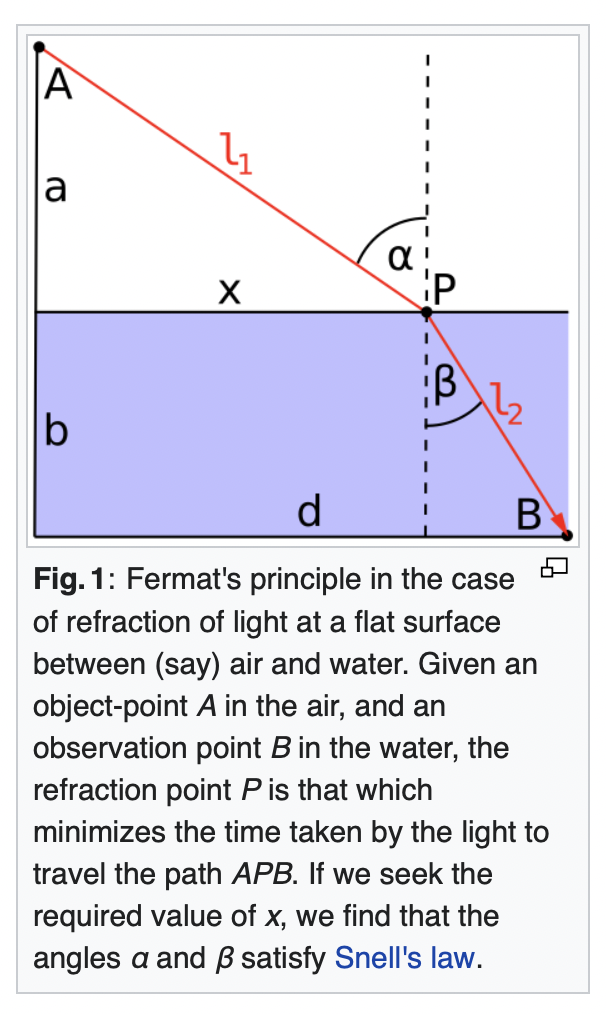
\includegraphics[width=1.3in]{Figures/fermat.png}
    \end{itemize}
  }

  \frame{
\vspace{-0.25in}
    \frametitle{Huygen's Principle: Path Integral}
    \begin{itemize}
        \item Kirchoff integral $A(\mu)=\int e^{i S(\theta,\mu)} d\theta$ 
        \item $S=\nu [(\theta-\mu)^2+\Psi(\theta)]$
        \item Highly oscillatory integral, even for $\Psi=0$
        \item Stationary phase points: $\partial_\theta S=0$ leads to (complex)
          Eikonal images $\theta_i$.
        \item flux/phase through curvature expansion (known as {\it
            steepest descent}): exact as $\nu \rightarrow \infty$
        \item Geometric limit considers only {\it Real} solutions $\theta_i$ and
      gives up phase
          information (length of trajectory)
        \item Geometric optics applicable at short wavelengths for
          extended sources
          (e.g. optical gravitational lensing of finite size sources,
          stars)     
    \end{itemize}
  }




  \frame{
\vspace{-0.25in}
    \frametitle{Optics: Geometric, Eikonal, Wave, P-L}
    \begin{itemize}
        \item Consider 1-D lens
        \item lensing potential $\Psi(\theta)$
        \item deflection $\Psi'$
        \item simplify for $D_{\rm ds}=\infty$
    \end{itemize}
\vspace{-0.5in}\hspace{2.5in}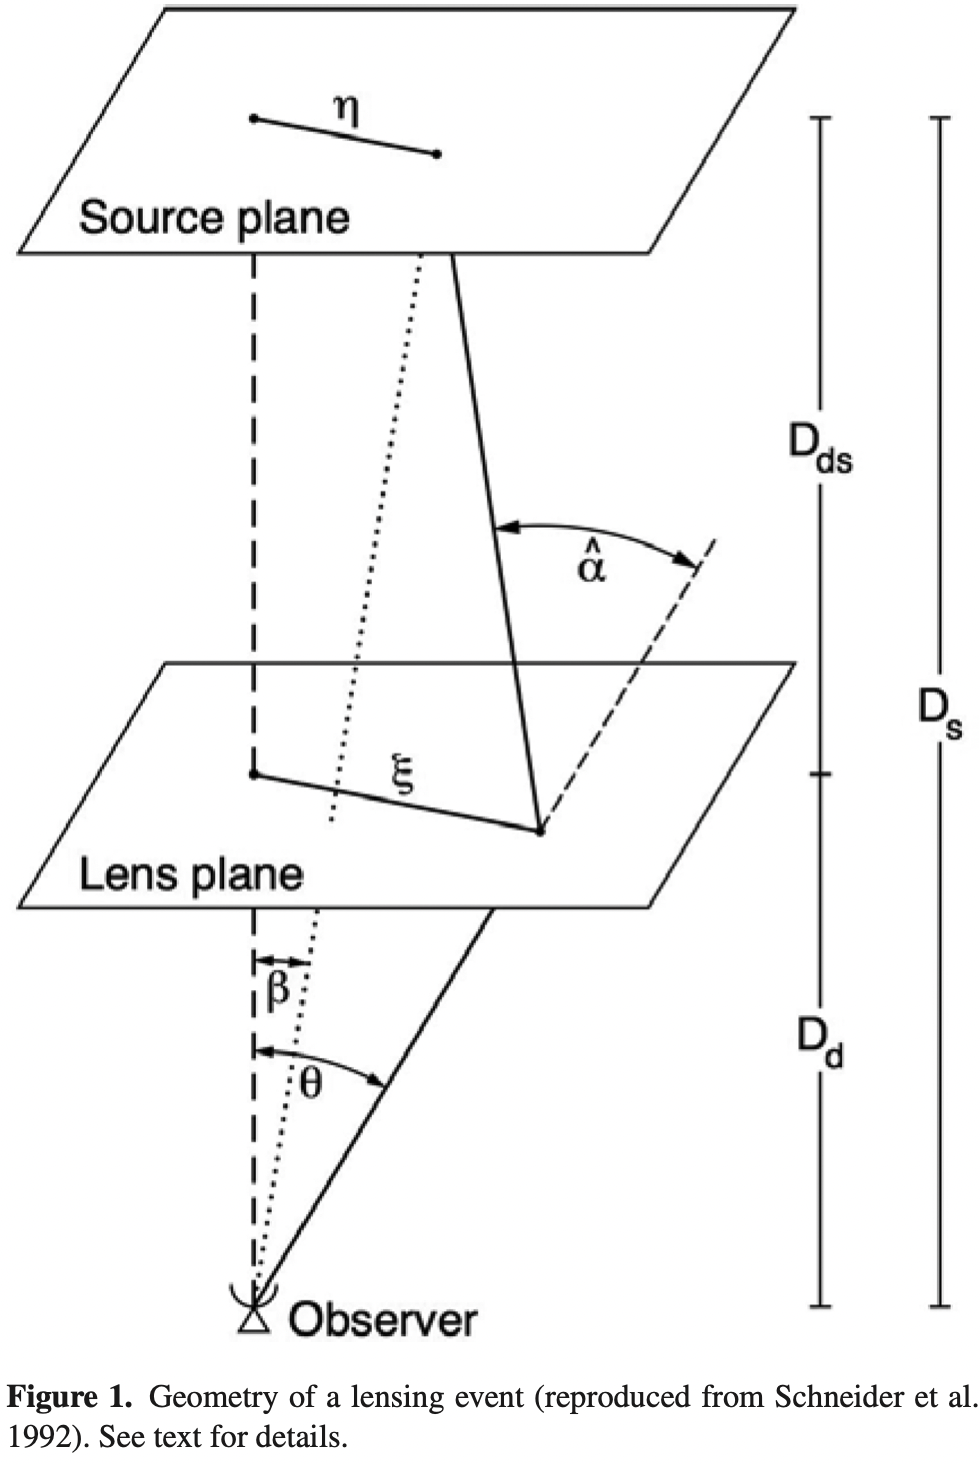
\includegraphics[width=1.5in]{Figures/lens.png}

  }




  \frame{
\vspace{-0.5in}
    \frametitle{Evanescent Images}
    \begin{itemize}
    \item consider ``rational lens'' potential $\psi(\theta)=\alpha/(1+\theta^2)$
    \item Geometric/eikonal images at $\psi'=\theta$
    \item 5 roots.  1 or 3 real roots, rest imaginary
    \item P-L: at most one imaginary image contributes!
    \item Resurgence theory to classify?
    \item Evanescent (imaginary) image can be brighter than unlensed real image
    \end{itemize}
  }


  \frame{
%\vspace{-0.5in}
    \frametitle{Rational 1-D lens}
\begin{center}
\includegraphics[width=3.1in]{Figures/theta-beta.eps}
\end{center}
  }

  
  \frame{
\vspace{-0.5in}
    \frametitle{Picard-Lefschetz Theory}
    \begin{itemize}
    \item descend integral along real line along Morse function Im(S)
    \item contour deforms into finite number of Thimbles of constant
      phase with maximum at saddle point (extrema $dS=0$)
    \item correctly identifies relevant saddle points
    \item resolves numerical challenges of oscillatory integral
    \item complex analysis works in multiple variables
    \item elevates concept of ``image'' deep into wave optics
    \item multiple public implementations (Feldbrugge+, Jow+)
    \end{itemize}
  }



  \frame{
\vspace{-0.5in}
    \frametitle{Picard-Lefschetz Theory}

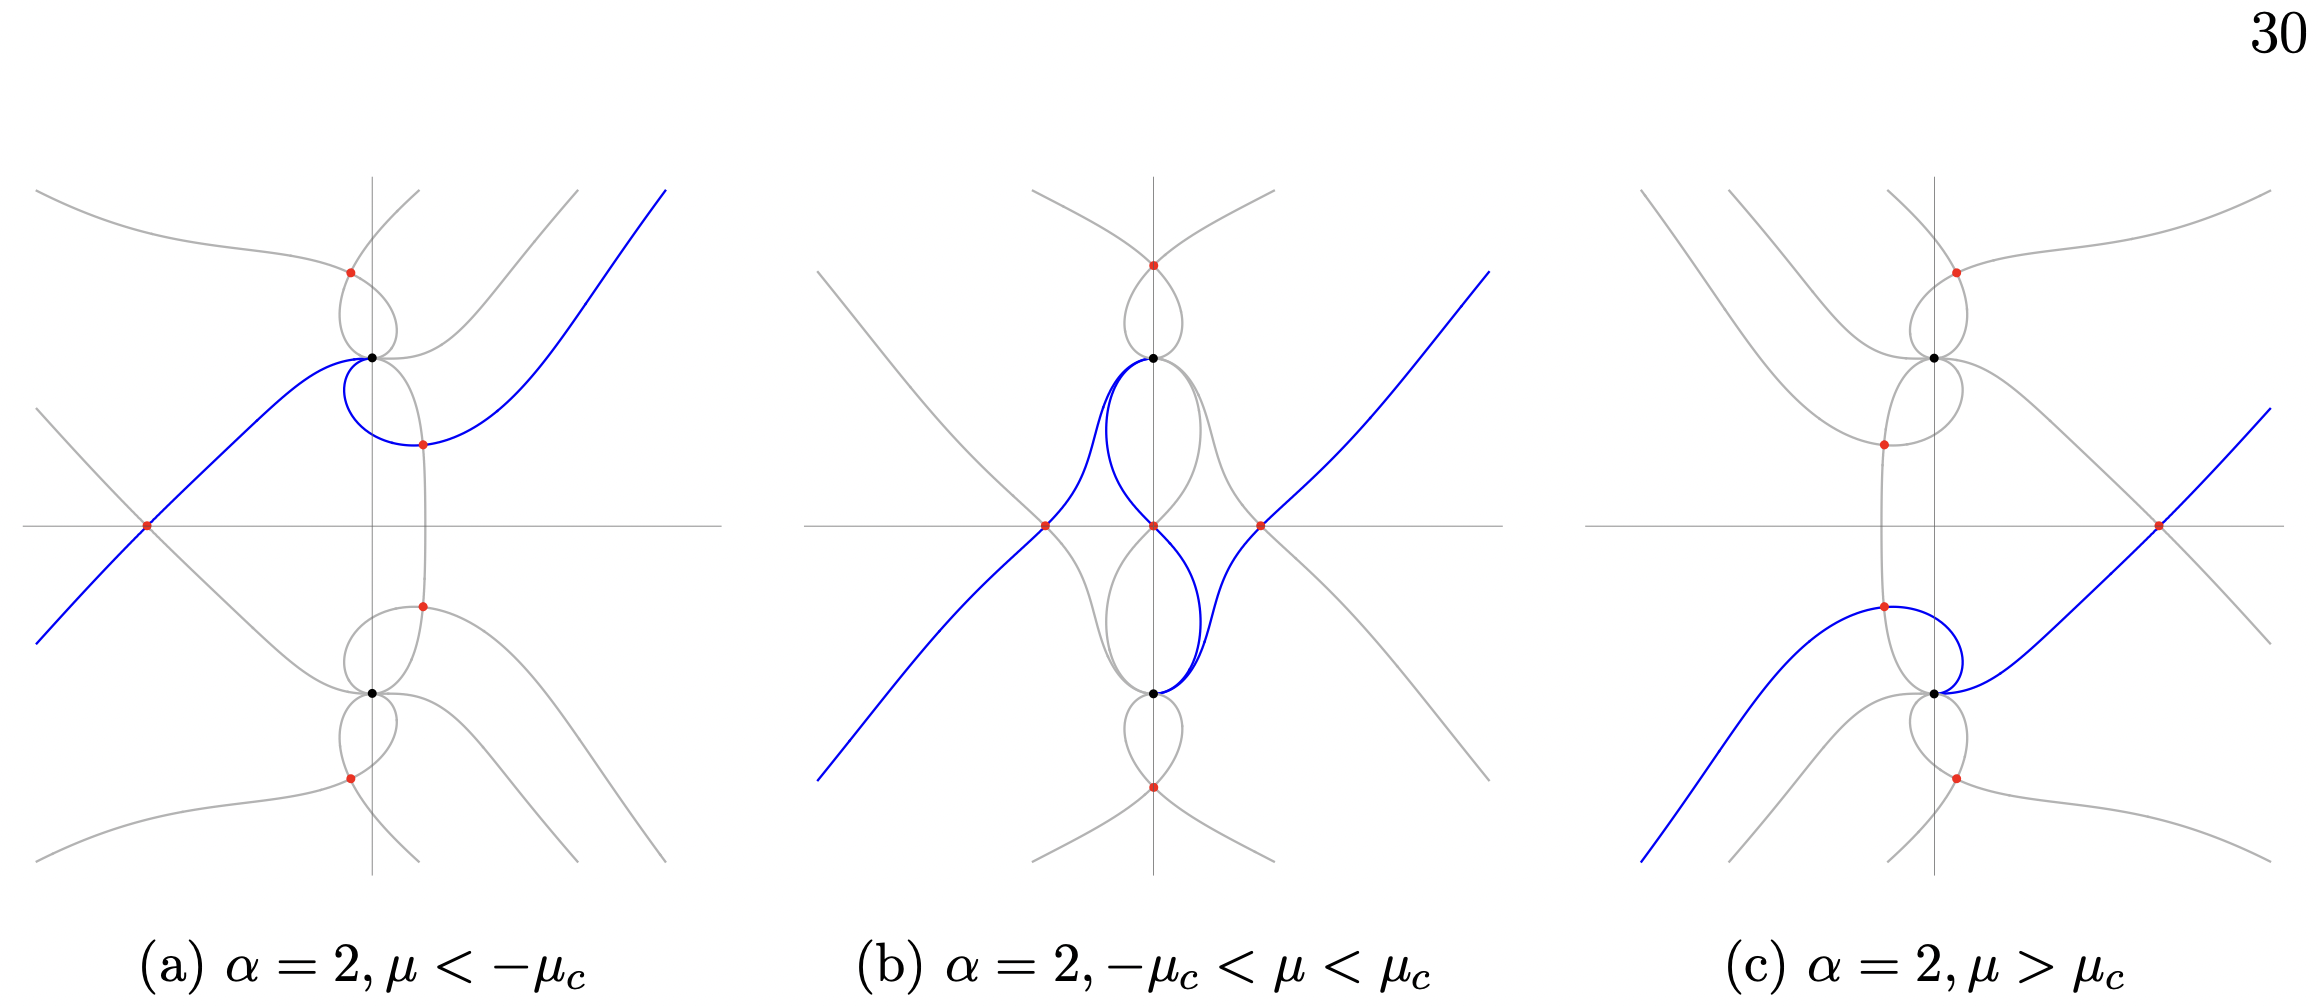
\includegraphics[width=4.5in]{Figures/thimbles.png}

Feldbrugge+2019
  }



 \frame{
\vspace{-0.5in}
    \frametitle{Quantum Mechanics}
    \begin{itemize}
    \item Feynmann path integral saddle points are similarly complex
    \item interprets tunneling as complex position path
    \end{itemize}
  }

  \frame{
%\vspace{-0.5in}
    \frametitle{Rosen-Morse Potential}
\begin{itemize}
\item $V(x)={\rm sech}^2(x)$
  \item  exactly solvable: 
$\sinh[x(t)]=\sqrt{\frac{1-E}{E}} \cosh[\sqrt{E}(t+t_0)]$
    \item for $\lim_{E\rightarrow 1+\epsilon^2} = \sinh^{-1} [\epsilon \sinh(t)]
$
    \end{itemize}
 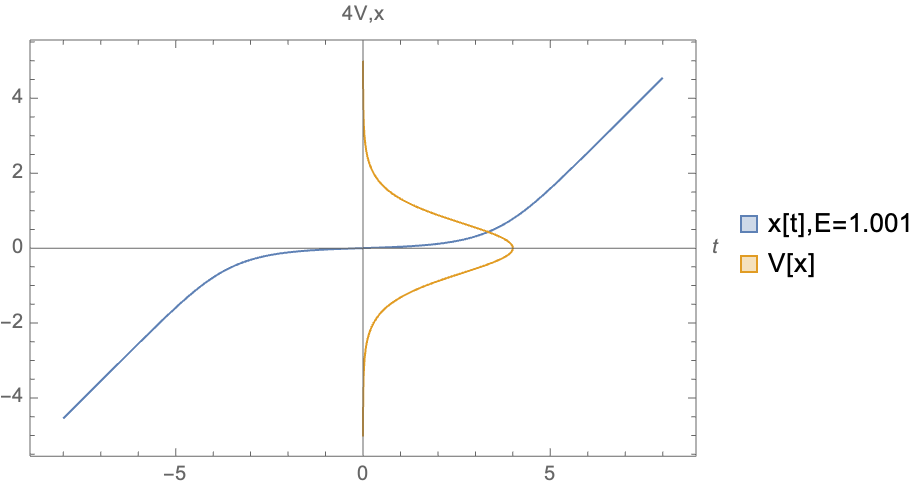
\includegraphics[width=3.5in]{Figures/sechreal.png}
  }



  \frame{
\vspace{-0.15in}
    \frametitle{Reinterpretation of Quantum Mechanics: 2309.12420 w/Feldbrugge, Jow}
\begin{figure}
        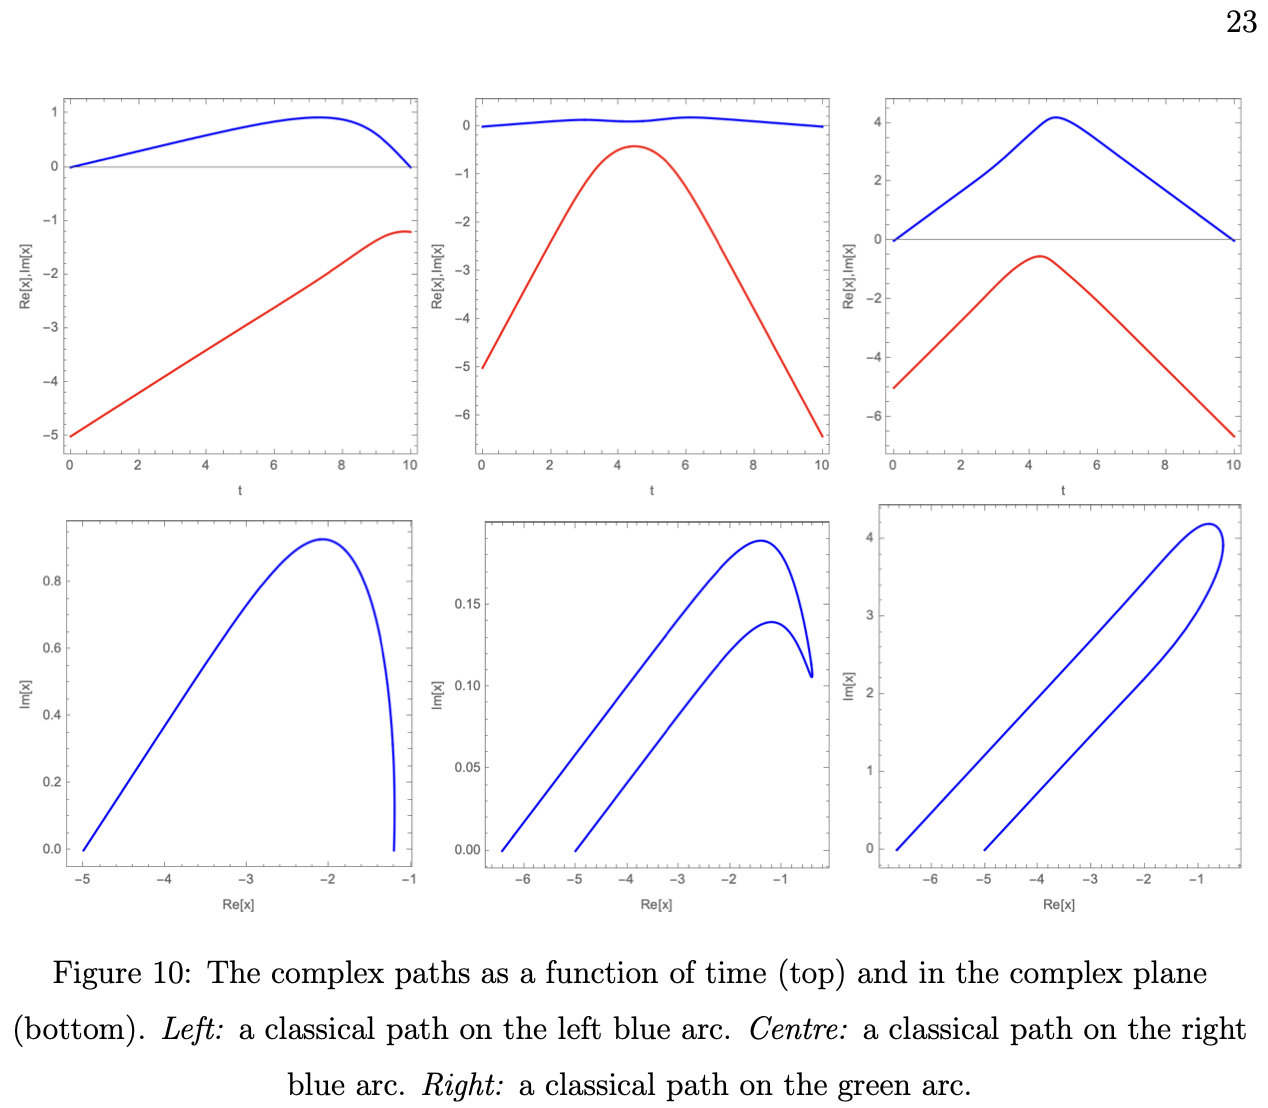
\includegraphics[width =0.8\textwidth]{Figures/saddle.png}
\end{figure}


  }


  \frame{
\vspace{-0.5in}
    \frametitle{Discussion}
    \begin{itemize}
    \item Eikonal effects applicable to compact radio sources,
      e.g. FRBs, pulsars
    \item full wave
effect dominates for long wavelengths as Fresnel scale is bigger then Einstein radius
    \item microlensing down to planet size
    \item gravitational waves:  LIGO, LISA, PTA
    \item with SKA PTA parameters and favourable source geometries, $H_0$
      measurement at 0.1\% possible.
      \item Shapiro delay uncertainty neglible
    \end{itemize}
  }



  \frame{
%\vspace{-0.5in}
    \frametitle{Conclusions}
    \begin{itemize}
     \item wave optics changes nature of astrophysical observables: Coherent FRB/pulsar/GW      radiation one of the potentially most
      precise measurements in physics
      \item PTA weak diffractive lensing may give new tool for Hubble
        Constant tension
      \item evanescent lensing/instantons
      \item evanescent lensing images understood through
        Picard-Lefschetz theory and complex/evanescent images
      \item at long wavelength, evanescent lensed images are unsuppressed
    \end{itemize}
  }

\end{document}
